% !TEX encoding = UTF-8 Unicode

\documentclass[a4paper]{article}

\usepackage{color}
\usepackage{url}
\usepackage[T2A]{fontenc} % enable Cyrillic fonts
\usepackage[utf8]{inputenc} % make weird characters work
\usepackage{graphicx}
\graphicspath{{slike/}}
\usepackage{amssymb}
\newcommand*{\field}[1]{\mathbb{#1}} % Set of Real numbers
\usepackage{amsmath}

\usepackage[english,serbian]{babel}
%\usepackage[english,serbianc]{babel} %ukljuciti babel sa ovim opcijama, umesto gornjim, ukoliko se koristi cirilica

\usepackage[unicode]{hyperref}
\hypersetup{colorlinks,citecolor=green,filecolor=green,linkcolor=blue,urlcolor=blue}

%\newtheorem{primer}{Пример}[section] %ćirilični primer
\newtheorem{primer}{Primer}[section]

\begin{document}

\title{Apstraktna interpretacija, osnovni pojmovi i primeri\\ \small{Seminarski rad u okviru kursa\\Verifikacija softvera\\ Matematički fakultet}}

\author{Milan Čugurović, 1009/2018\\ milan\_cugurovic@matf.bg.ac.rs}
\maketitle

\abstract{
Cilj ovog rada jeste prevashodno razumevanje pojma apstrakcije u kontekstu statičke analize i programerske interpretacije istog termina. Kroz niz slikovitih i konkretnih primera ovaj rad pokučava da objasni i intuitivno prbliži čitaocima jednu kompleksnu oblast, inicijalno osmišljenu po idejama Patrika Kusota. }

\tableofcontents

\newpage

\section{Uvodni primeri}
\label{sec:uvod}
Dora Mar (rođena kao Henrite Teodora Marković, Tur 1907. - Pariz, 1997.), bila je poznata francuska slikarka, fotograf i pesnik. Ćerka poznatog hrvatskog arhitekte Josipa Markovića iz Siska poznata je i kao muza slikara Pabla Pikasa, koji ju je portretisao na brojnim portretima tokom njihove burne ljubavne veze tokom 1930ih.\cite{dora} \newline
Dorina fotografija, kao i par Pablovih portreta iste dati su na slici  \ref{fig:doramar}.
\begin{figure}[h!]
\begin{center}
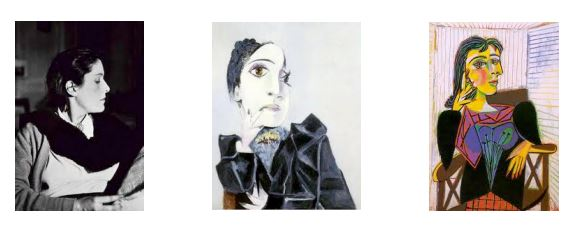
\includegraphics[scale=0.6]{doramar.JPG}
\end{center}
\caption{Originalna fotografija i apstrakcije umetnika}
\label{fig:doramar}
\end{figure} \newline 
Na ovoj slici vidimo prikaz modela kao nematerijalan i sa naglašenim akcentom na apstrakciju. Vidimo umetnikovu sposobnost da savlada konkretno i ogoli suštninu, kako fizičkog izgleda, tako i karaktera naslikane dame.\cite{pcousot3}\newline

Decembra 1945. godine nastaje čuveni Pikasov 'Bik'. (slika \ref{fig:bull}) 'Bik' jeste serija litografija, u kojoj se kroz svaku sledeću sliku umetnik trudi da otkrije svoje suštinsko prisustvo kroz progresivnu analizu oblika. Svaka ploča je sukcesivna faza u traganju za duhom zveri. Počevši od sveže i spontane, pre svega realistične slike zivotinje, dolazimo do jednostavnih linija u kojima je sažeta sva suština kompletne serije, kompletan razvoj, i kojom Pikaso hvata apsolutnu suštinu stvorenja u svega par linija.\cite{bull}
\begin{figure}[h!]
\begin{center}
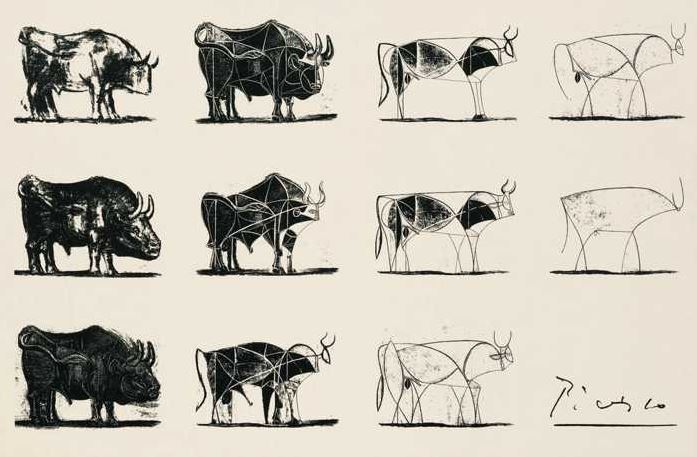
\includegraphics[scale=0.51]{bull.JPG}
\end{center}
\caption{'Bik', 1945, serija litografija}
\label{fig:bull}
\end{figure} \newline

Slika \ref{fig:miles} krije jednu zanimljivu andegdotu američkog blogera Endija Bejoua. Naime, čuveni fotograf Dzej Mejsel tužio je blogera zbog upotrebe pikselizovane verzije slike omota albuma 'Kind of Blue', koju je Mejsel slikao 1967. godine. Prema Mejselovim advokatima, pikselizovana slika slike jeste i dalje upotreba originalne fotografije. Bloger i fotograf su se nagodili, s tim da je Endi morao da isplati 32.500 dolara fotografu.\cite{pixel} \newline
\begin{figure}[h!]
\begin{center}
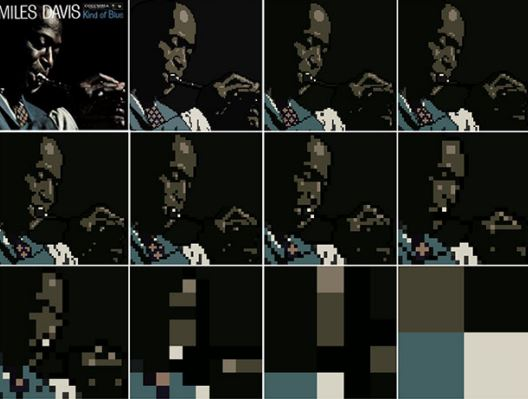
\includegraphics[scale=0.6]{miles.JPG}
\end{center}
\caption{Majls Dejvis, 'Kinds of blue', omot albuma i pikselizacija}
\label{fig:miles}
\end{figure}

Razmislimo malo o pojmu apstrakcije figura u ravni. Slika \ref{fig:numeric} predstavlja načine na koje uspevamo da opisemo odnosno apstrahujemo formulama skupove tačaka u ravni koje vizuelno opažamo. Formule kojima ih opisujemo izdvajaju suštinu ovih skupova, u najužem smislu.
\begin{figure}[h!]
\begin{center}
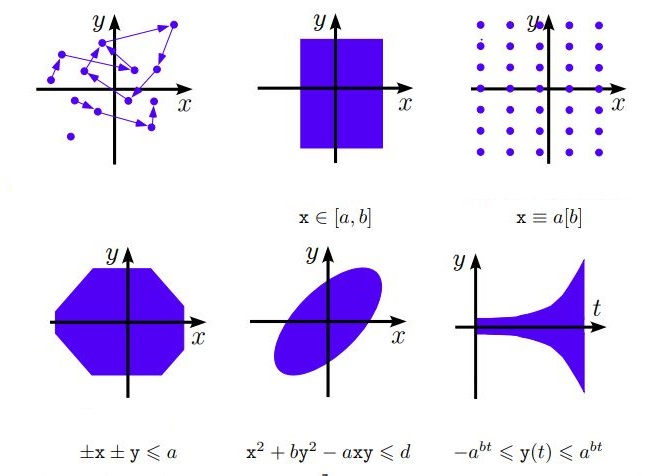
\includegraphics[scale=0.5]{numeric.JPG}
\end{center}
\caption{Apstrakcija fugura u ravni}
\label{fig:numeric}
\end{figure}\newline
Na prethodnoj slici redom pokušavamo da matematički opišemo, odnosno da apstrahujemo skupove tačaka u ravni, koji predstavljaju nešto što nam je poznato kao putanja, interval, celobrojna mreža (prvi red, sa leva na desno), oktagon, elipsa i eksponencijalna kriva (drugi red, isti pravac).


\section{Detaljniji primer - skup funkcija}
\subsection{Matematički pristup}

Razmotrimo sledeću situaciju. Pred nama se nalazi skup funkcija 
$f_i: \field{R} \rightarrow \field{R}.$ Potrebno je na neki način opisati ovaj skup. Kako je domen svake od funkcija skup realnih brojeva, jasno je da se zadatak svodi na opisivanje njihovih kodomena. Primer skupa funkcija dat je na slici \ref{fig:f1}.
\begin{figure}[h!]
\begin{center}
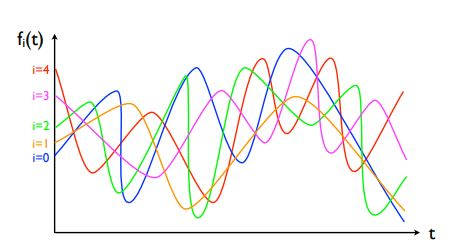
\includegraphics[scale=0.4]{f1.JPG}
\end{center}
\caption{Skup funkcija}
\label{fig:f1}
\end{figure} \newline
Prva stvar koju primećujemo jeste da je skup funkcija sa slike ograničen (u smislu kodomen svake od funkcija je ograničen). Odlično! To nam odmah daje sledeću ideju. Hajde da nađemo minimalnu vrednost $m$ koju neka od funkcija dostiže, analogno nađemo $M$ koje predstavlja najveću vrednost koju neka od njih dostiže, i onda je jasno, naš skup apstrahovan pravougaonikom $t \times [m, M]$. \newline
Dakle, uspeli smo da nađemo jednu apstrakciju zadatog nam skupa. Međutim, prva stvar koja svakom matematičaru zapada za oko jeste nepreciznost našeg rešenja. \footnote{Zamislimo samo skup funkcija $f_i, i=1,...,100$, gde je svaka od ovih funkcija dobijena kada se na sinusoidu uniformno doda ograničen šum. Tada naša aproksimacija, jasno, jeste pravougaonik $t \times [-1,1]$. Međutim, veliki deo našeg pravougaonika je zapravo prazan!} Zaključujemo, trebamo nekako profiniti naše rešenje. \newline
Svakome ko je nekada slušao makar i uvodni kurs matematičke analize, ideja koja prva pada na pamet jeste ideja integralnih suma. Naime, hajde da domen načih funkcija izdelimo na manje delove, segmente, i onda istu ideju kao malopre primenimo na svakom segmentu. U zavisnosti od podele domena na segmente, dobijamo apstrakcije kao na slici \ref{fig:f234}.
\begin{figure}[h!]
\begin{center}
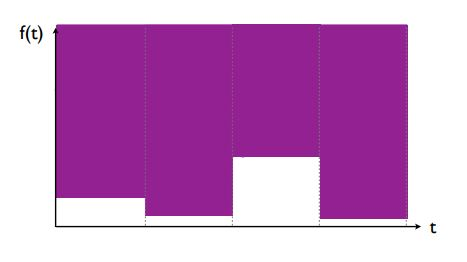
\includegraphics[scale=0.3]{f2.JPG}
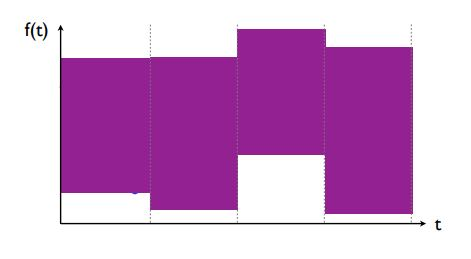
\includegraphics[scale=0.3]{f3.JPG}
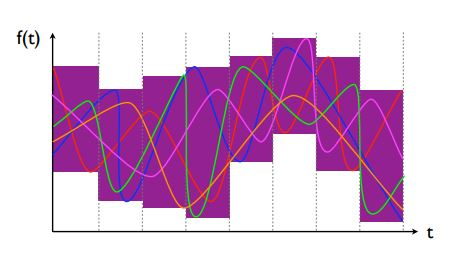
\includegraphics[scale=0.3]{f4.JPG}
\end{center}
\caption{Preciznija apstrakcija}
\label{fig:f234}
\end{figure} \newline
Dalje se postavlja pitanje gde je granica. U smislu, do koje mere mogu da usitnim segmente na kojima tražim ekstremne vrednosti $m$ i $M$. Na slici \ref{fig:f56} prikazana je jedna jos sistnija podela (u smislu dužine segmenata), kao i granični slučaj (slučaj kada dužina segmenata na koje delim domen teži nuli).
\begin{figure}[h!]
\begin{center}
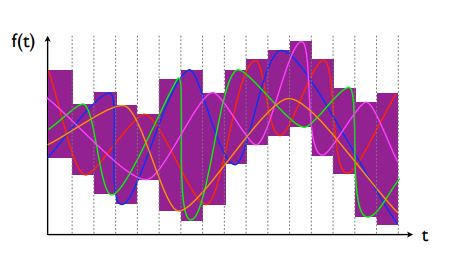
\includegraphics[scale=0.3]{f5.JPG}
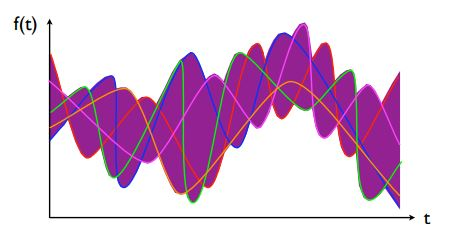
\includegraphics[scale=0.3]{f6.JPG}
\end{center}
\caption{Finija podela - finija apstrakcija}
\label{fig:f56}
\end{figure} \newline
Jasno, na svakom od segmenata, nač skup funkcija ne moramo ograničavati tako što ga smestimo u pravougaonik, možemo prosto koristiti funkcije koje nisu prave paralelne $Ox$ osi. Jedan primer takve aproksimacije dat je na slici \ref{fig:f78}. Bitno je primetiti da ovakva apstrakcija nije uporediva (u smislu inkluzije sa prethnodnim apstrakcijama pravougaonicima). Na istoj slici data je i hijerarhija dosadašnjih apstrakcija.
\begin{figure}[h!]
\begin{center}
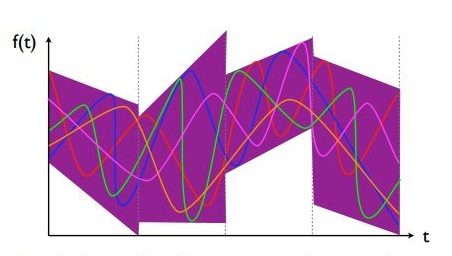
\includegraphics[scale=0.4]{f7.JPG}
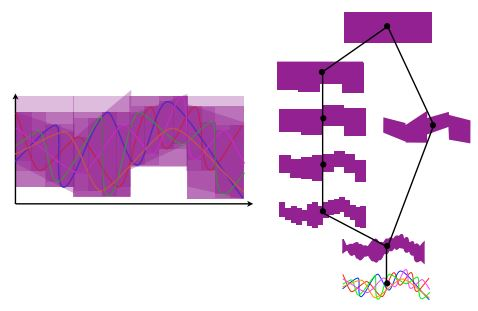
\includegraphics[scale=0.4]{f8.JPG}
\end{center}
\caption{Hijerarhija apstrakcija}
\label{fig:f78}
\end{figure} \newline

\subsection{Programerski pristup}

Počevši od nekoliko neformalnih primera koji se odnose na slikarstvo, litografiju i pikselizaciju slika, preko matematičhih primera iz Dekatrove ravni, došli smo do pojma apstrakcije skupa funkcija, odnosno do aproksimacije istog skupa. Prethodna dva termina, apstrakcija i aproksimacija, ispostavljaju se jako bitnim, i jako povezanim u jednoj od oblasti statičke analize softvera, koja i nosi naziv Apstraktna interpretacija. \newline

Primer iz prethodnog odeljka ispostavlja se kao jako bitan i jako slikovit prikaz tehnika apstrakte interpretacije. Zamislimo da imamo nekakv program (linije koda) na nekoj mašini, kog izvršavamo više puta, sa raznim ulazima. Program ima puno poziva raznih funkcija, grananja, uslovnih izvršavanja. Na koji način možemo predstaviti razne putanje kojima prolazimo kroz program ovim izvršavanjima? \newline

Odgovor na ovo pitanje krije se u narednom poglavlju rada.

\section{Apstraktna interpretacija}

\subsection{Motivacija}

Evolucija hardvera za faktor $10^n$ u poslednjih četrdeset godina dovela je do enormnog povećanja veličine i kompleksnosti softvera. Broj oblasti u kojima su veoma veliki programi (u smislu broja linija koda, od 1 do 50 miliona linija) postali primenljivi, a često i neophodni, sve je više. Cena pisanja programa ovakvih gabarita mora biti razumna, kao i dalje odrzavanje i modifikovanje u toku životnog ciklusa istog (što je obično od dvadeset do trideset godina). Efikasnost programiranja i veličina timova koji pomenuti softver kreiraju i održavaju očigledno ne može da isprati ovaj rast (čak ni na logaritamskoj skali). Broj grešaka po liniji koda, sa povećanjem veličine koda eksponencijalno raste, pa je stoga njihovo otklanjanje i verifikacija softvera izuzetno otežana. Zbog svega ovoga, pitanje pouzdanosti softvera postalo je glavni izazov u modernim programerskim zajednicama. \newline

Alati i tehnike verifikacije koje se zasnivaju na izvršavanju ili simuliranju izvršavanja programa za što veći broj ulaza, jasno gube bitku sa novim gigantima. Cena debagovanja kompajliranog koda ili simulacija izvršavanja istog drastično raste porastom broja linija, i kao po pravilu vodi do male pokrivenosti. \newline

Formalne metode verifikacije softvera pokušavaju da dokažu korektnost programa za sve moguće ulaze. One uključuju deduktivne metode, proveravanje modela, i statičku analizu programa. \newline

Konkretna semantika programa formalizuje (predstavlja matematički model) skupa svih mogućih izvršavanja i stanja programa. Konkretna semantika programa jeste jedan matematički beskonačan objekat, u smislu da \textbf{nije izračunljiv}: nije moguće napisati program koji može da reprezentuje i izračuna sva moguća izvršavanja proizvoljnog programa za sve moguće ulaze.
Sva netrivijalna pitanja vezana za konkretnu semantiku programa su \textbf{neodličiva}: nije moguće napisati program koji može da odgovori na svako pitanje vezano za sva moguća izvršavanja nekog programa (konkretna semantika ovog programa morala bi biti izračunljiva).

\begin{primer}
Matematička analogija jeste da ne postoji dokazivač teorema koji može da dokaže proizvoljnu teoremu aritmetike, bez ljudske pomoći.
\end{primer}

\begin{primer}
(Kurt Gedel) Razmotrimo pitanje da li se program za zadati ulaz završava ili ne. Pretpostavimo da se program termination(P) uvek završava, i da vraća tačno ako se program P završava za sve ulaze, inače vraća netačno. Tada nas program \begin{quote}
    P $\equiv$ while termination(P) continue
\end{quote} vodi do kontradikcije.
\end{primer} 

Neodlučivost i kompleksnost izračunavanja u alatima za verifikaciju softvera prevazilaze se korišćcenjem raznih aproksimacija. Ovo znači da će se pomenuti alati koji defakto imaju svoja vremenska i prostorna ograničenja u praksi ili oslanjati na odredjene hipoteze o konačnosti izracunavanja ili nuditi nepotpuna rešenja koja zahtevaju interakciju korisnika ili moći da proveravaju samo ogranicene delove specifikacije programa. Cilj apstraktne interpretacije jeste da formalizuje ove aproksimacije u jedinstven framework.\cite{pcusot} \cite{prcousot}

\subsection{Osnovni pojmovi}
    
Kako se verifikacija softvera bavi karakteristikama, odnosno skupovima (objekata sa tim karakteristikama), to se apstrakna interpretacija može formulisati nezavisno od konteksta, kao teorija aproksimacije skupova i skupovnih operaciija (naravno, može uključiti i induktivne definicije kao i svaka teorija skupova). Drugi način formulisanja apstraktne interpretacije jeste gledanje na nju kao na teoriju aproksimacija ponašanja dinamičkih diskretnih sistema (npr. semantike programa). Kako ovakva ponašanja mogu biti karakterisana fiksnim tačkama (ovo odgovara iteraciji) to je ključni deo obezbediti konstruktivne i efektivne metode za aproksimiranje fiksih tačaka i proveru istih apstrakcijom.

\subsubsection{Semantika fiksnih tačaka}

Semantika programskog jezika definiše semantiku za sve programe napisane u tom jeziku. Semantika programa definiše formalni matematički model svih mogućih ponašanja računarskog sistema koji izvršava taj program, u interakciji sa proizvoljnim ulazom. Kako bi se uporedile semantike raznih programa pokazuje se da se semantika jednog programa moze hijerarhijski organizovati po slojevima apstrakcije.

\subsubsection{Semantika putanja}

Detaljniji pristup ispitivanju izvršavanja programa jeste takozvano praćenje putanja. Jedno izvršavanje programa za dati ulaz (u smislu date interakcije sa okruženjem) jeste sekvenca stanja u kojima se sistem nalazi, posmatranih u diskretnim intervalima vremena, počevši od inicijalnog, početnog stanja, krećući se iz jednog stanja u drugo izvršavanjem atomičnog skupa insreukcija programa ili naredbom skoka, na kraju završavajući u terminišućem tj. završnom stanju ili stanju greške (eventualno završavajući u neterminišućem stanju, u kom slučaju je putanja beskonačna), videti sliku \ref{fig:path}.
\begin{figure}[h!]
\begin{center}
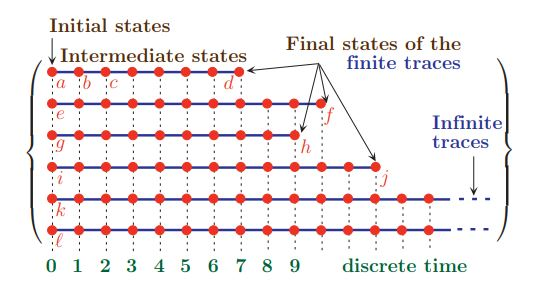
\includegraphics[scale=0.7]{path.JPG}
\end{center}
\caption{Primeri računanja putanja}
\label{fig:path}
\end{figure} \newline

\subsection{Osnovni pojmovi kroz paktičan primer}

Svojstvo \textit{sigurnosti} programa kaže da ni jedno izvršavanje programa (za proizvoljni ulaz i proizvoljnu interakciju sa okruženjem) neće program dovesti u stanje greške. Dokaz da program ima pomenuto svojstvo sigurnosti sastoji se od pokazivanja da je presek semantike programa i zabranjene zone (zone greške) prazan. Naravno, i ovo je jedan neodlučiv problem (semantika programa nije izračunljiva). Stoga je nemoguće doći do preciznog odgovora sa računarom koji raspolaže konačnim resursima, i bez ljudske interakcije.\cite{pcousot2} Slika \ref{fig:graf12} prikazuje moguće putanje jednog programa, kao i zabranjenu zonu.
\begin{figure}[h!]
\begin{center}
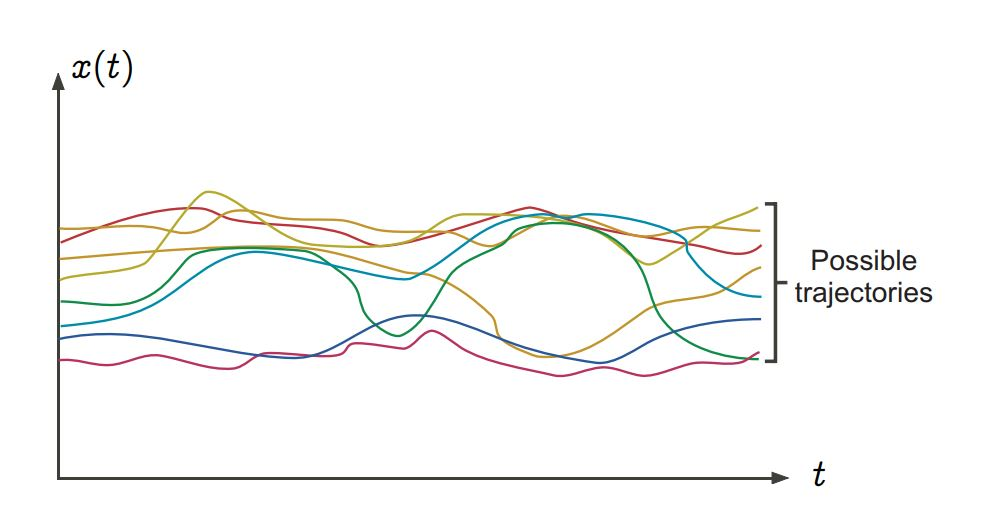
\includegraphics[scale=0.2]{graf1.JPG}
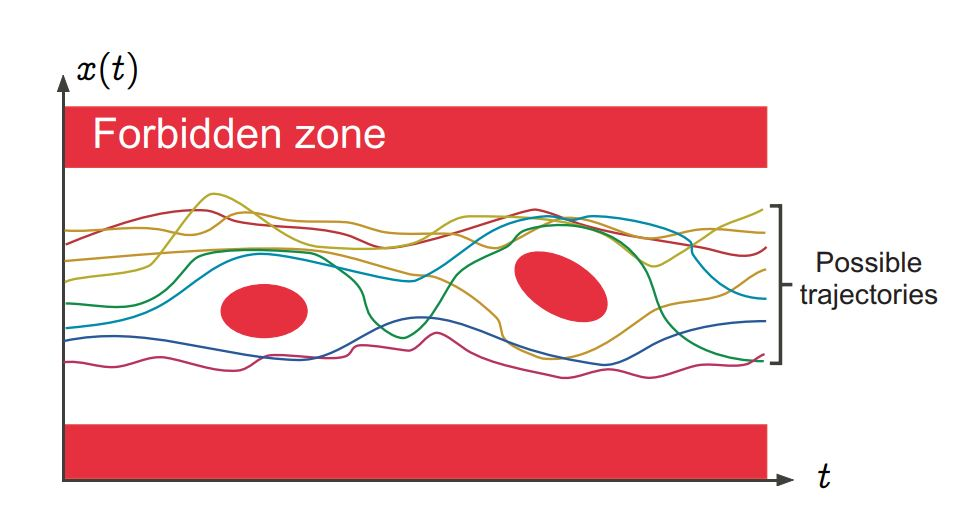
\includegraphics[scale=0.2]{graf2.JPG}
\end{center}
\caption{Primeri putanja programa; zabrnjena zona}
\label{fig:graf12}
\end{figure} \newline

Jedan pristup odredjivanju preseka izmedju svih mogućih putanja programa i zone greške jeste testiranjem. Testiranje se sastoji u razmatranju podskupa svih mogućih putanja. Ono nije dokaz korektnosti, već samo pokušaj pronalaska preseka pomenutih skupova ili dostizanja određenog stepena poverenja u sistem koji se testira. Primer testiranja dat je na slici \ref{fig:graf3}.
\begin{figure}[h!]
\begin{center}
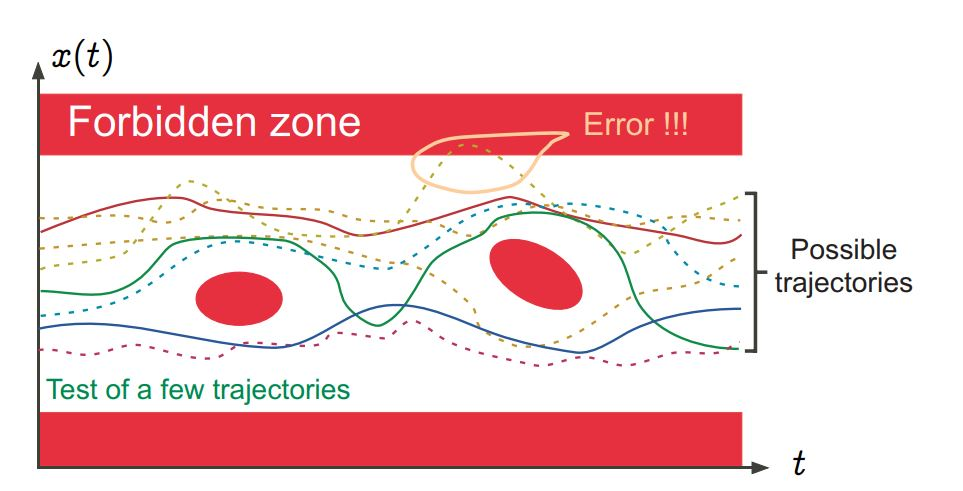
\includegraphics[scale=0.3]{graf3.JPG}
\end{center}
\caption{Testiranje ispitivanjem nekih konkretnih putanja}
\label{fig:graf3}
\end{figure} \newline

Apstraktna interpretacija sastoji se u odredjivanju i razmatranju \textit{apstraktne semantike}, koja predstavlja nadskup konkretne semantike programa. Konkretna semantika programa (koja se opisuje konkretnim domenom i relacijama nad tim domenom) može biti previše kompleksna (posebno za velike programe s obzirom da je ispitivanje da li neko svojstvo važi nad ogromnim domenom skupo zbog veličine samog domena, odnosno zbog velikog broja putanja kroz program, kao i zbog neodlučivosti koja se javlja u raznim kontekstima). Umesto razmatranja konkretnog domena, razmatra se domen apstraktne semantike programa, koji iako nije tako precizan kao konkretni domen, može u nekim situacijama dati odgovore o važenju nekih svojstava. Važno je da je konkretni domen podskup apstraktnog domena, odnosno ako se dokaže ispravnost programa u apstraktnoj semantici, onda ta ispravnost važi i u konkretnoj semantici (u smislu ako je apstraktna semantika sigurna tj. ako ona nema preseka sa zonom greške, onda je takva i konkretna semantika programa). \footnote{Primere koji detaljnije opisuju odnos između konkretne i apstraktne sematike prgrama, kao i odnose koji važe između pomenutih možete videti u primerima koji se nalaze u poglavlju četiri.} Primer apstrakcije trajektorija prikazan je na slici \ref{fig:graf4}.
\begin{figure}[h!]
\begin{center}
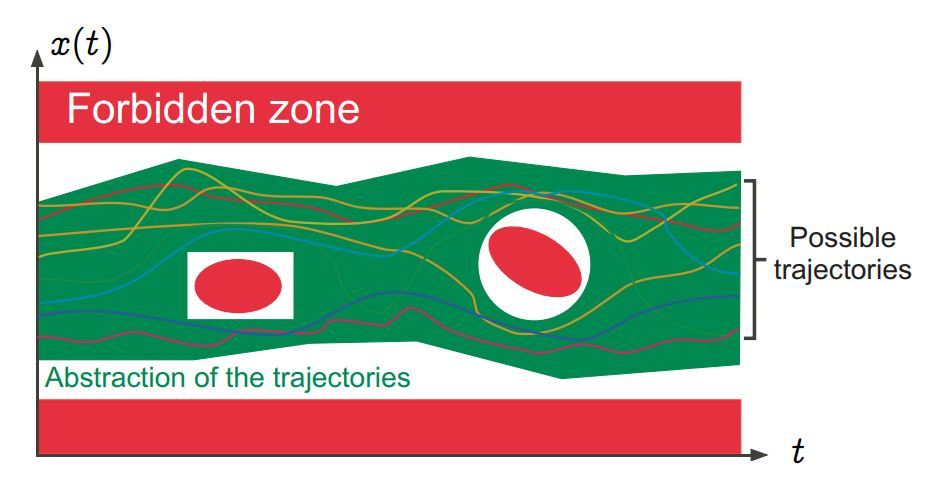
\includegraphics[scale=0.35]{graf4.JPG}
\end{center}
\caption{Odnos apstraktne i konkretne semantike}
\label{fig:graf4}
\end{figure} \newline

Formalne metode koje predstavljaju apstraktnu interpretaciju razlikuju se u načinu kojim dolaze do apstraktne semantike: 
\begin{itemize}
    \item \textbf{Proveravanje modela}: apstraktnu semantiku zadaje direktno korisnik; može biti izvršena automatski, tehnikama relevantnim za statičku analizu
    \item \textbf{Deduktivne metode}: apstraktna semantkia je definisana uslovima verifikacije odnosno korisnik mora da obezbedi apstraktnu semantiku; takođe može biti izvršena automatski, tehnikama relevantnim za statičku analizu
    \item \textbf{Statička analiza}: apstraktna semantika se računa automatski iz programskog koda prema predefinisanim pravilima apstrakcije (koja nekada mogu biti posebno prilagođavana bilo od strane korisnika, bilo automatski)
\end{itemize} 

Apstraktna semantika mora obezbediti da se otkriju sve moguće greške, pri tom se teži da ista bude što je moguće preciznija (da se izbegnu lažna upozorenja), kao i da bude što jednostavnija (da se izbegnu računski problemi). Na slikama koje slede prikazane su najpreciznija moguća apstrakcija (slika \ref{fig:graf5}), apstrakcija koja dovodi do greske i apstrakcija koja ispravlja tu grešku (slika \ref{fig:graf67}), kao i apstrakcija koja proizvodi lažna upozorenja (slika \ref{fig:graf8}).

\begin{figure}[h!]
\begin{center}
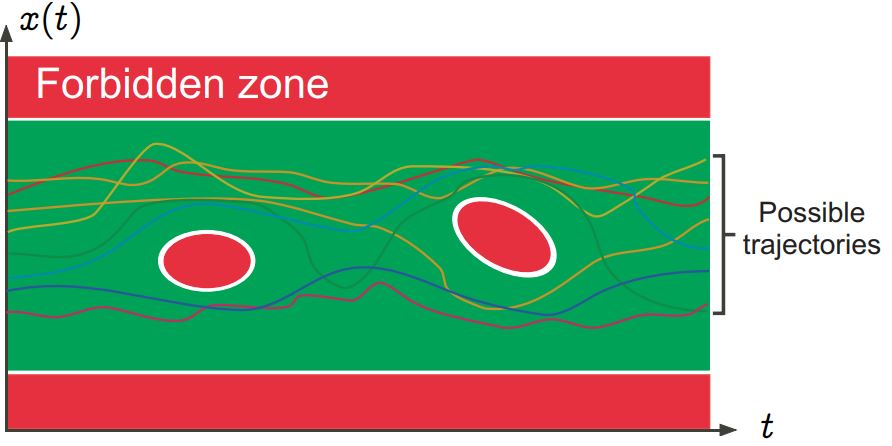
\includegraphics[scale=0.3]{graf5.JPG}
\end{center}
\caption{Najpreciznija moguća apstrakcija}
\label{fig:graf5}
\end{figure}

\begin{figure}[h!]
\begin{center}
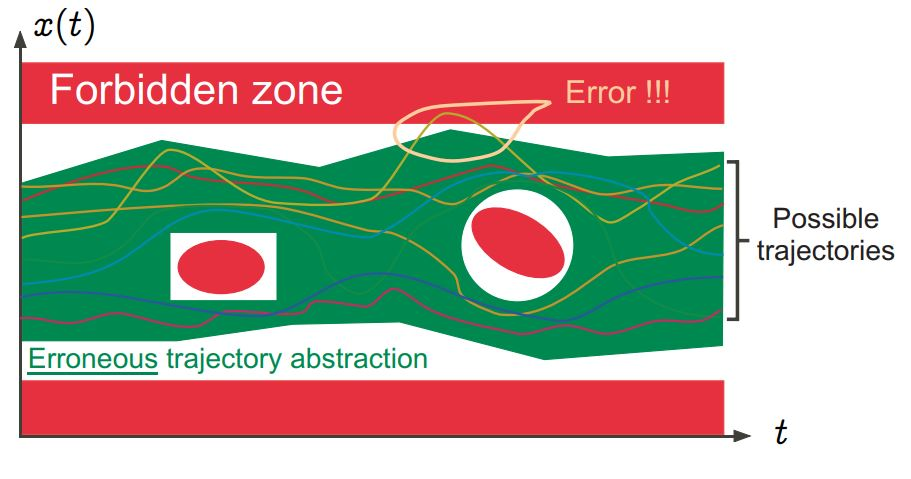
\includegraphics[scale=0.2]{graf6.JPG}
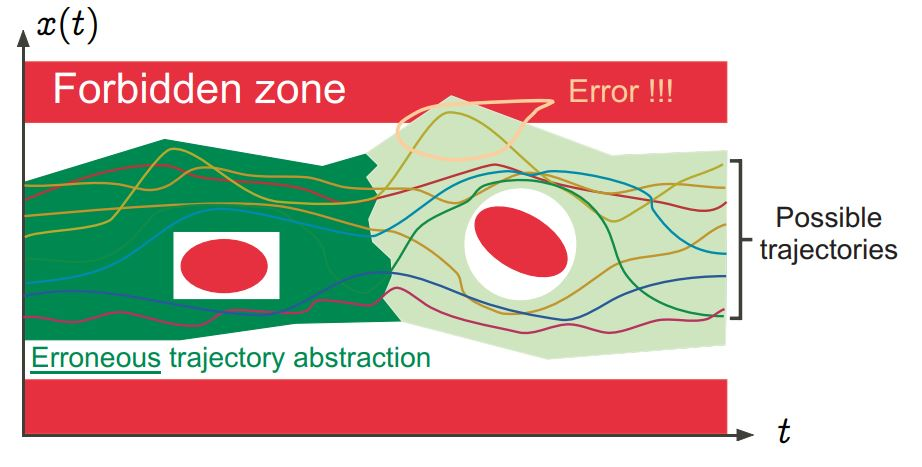
\includegraphics[scale=0.2]{graf7.JPG}
\end{center}
\caption{Greška i njena ispravka}
\label{fig:graf67}
\end{figure} 

\begin{figure}[h!]
\begin{center}
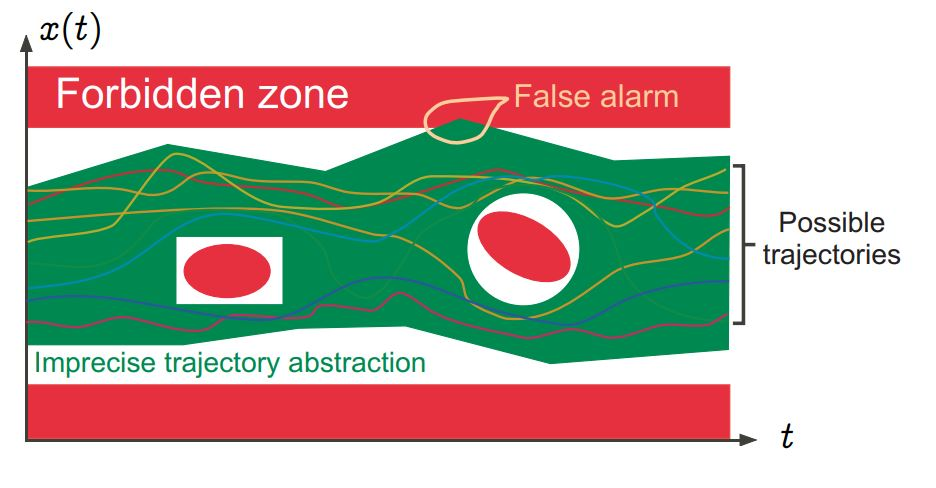
\includegraphics[scale=0.3]{graf8.JPG}
\end{center}
\caption{Lažno upozorenje}
\label{fig:graf8}
\end{figure} 


\section{Par konkretnih primera}
\subsection{Parnost broja}

Prodiskutujmo problem određivanja parnosti datog broja. Konkretna interpretacija ovog problema odnosila bi se na rešavanje problema proveravanjem ostatka pri deljenju sa sva datog broja. Apstraktna interptetacija bi, sa druge strane, problem svela na proveravanje poslednje cifre datog nam broja, i u zavisnosti od iste, odredili bi parnost. Konkretan domen problema u ovom slučaju jeste skup prirodnih brojeva $\field{N}$, dok je apstraktni domen znatno manji, cifre od 0 do 9. Svaki broj se preslikava u svoju poslednju cifru. \newline

Vezano za prethodno, primetimo par stvari. Razmatranje poslednje cifre, je u opštem slučaju dosta efikasnije od deljenja sa dva. Dalje, apstraktni domen nije tako precizan kao konkretan domen, ali daje odgovore na pitanje parnosti broja. Ispitivanje nad konkretnim domenom, koje je otežano veličinom istog (skupo deljenje velikih brojeva) prevazilazi se apstrakcijom konkretnog domena, odnosno konkretan domen tj. skup $\field{N}$ zamenjuje se apstraktnim domenom opisa ovih vrednosti tj. ciframa od 0 do 9.

\subsection{Svojstvo deljivosti sa tri}

Razmotrimo problem ispitivanja da li je dati broj iz intervala [0, 1 000 000 000] deljiv sa tri. Konkretna interpretacija proveravala bi ostatak datog broja pri deljenju sa tri. Apstraktna interpretacija računala bi zbir cifara, koji je dosta manji broj nego original, pa bi njega delili sa tri. Svaki broj se dakle preslikava u zbir svojih cifara. Konkretan domen jeste skup prirodnih brojeva iz intervala [0, 1 000 000], dok je apstraktni domen skup brojeva iz intervala [0, 81]. Drugi pristup je u opštem slučaju efikasniji od prvog. \newline

Dodatno, važe i sva svojstva koja karakterišu apstraktnu interpretaciju, a koja su navedena u prethodnom primeru.

\subsection{Znak broja}

Razmotrimo problem određivanja znaka datog nam celog broja. \cite{mvj}
Konkretan domen problema jeste beskonačan, radi se o skupu celih brojeva. On se može zameniti apstraktnim domenom koji sadrži vrednosti znakova brojeva, odnosno skupom \{+, -, 0\}. Time dolazimo do sledećeg skupa apstrakcija: 
\begin{align*}
    a_0 &= \{0\} \\
    a_+ &= \{n|n>0\} \\
    a_- &= \{n|n<0\}
\end{align*}

Ovakva apstrakcija može da nam da potpuno precizan odgovor na pitanje znaka proizvoda dva broja. Naime:
\begin{align*}
    0 \times a_+ &= 0 \times a_- = a_+ \times 0 = a_- \times 0 = 0 \\
    a_+ \times a_+ &= a_- \times a_- = a_+ \\
    a_+ \times a_- &= a_- \times a_+ = a_-
\end{align*}

Na osnovu prethodna dva primera, kao i dosadašnjeg dela ovog primera, neko bi pomislio, pa super nama apstraktni domen može dati odgovor na sve što nas zanima, pritom je dosta jednostavniji od konkretnog domena. Nažalost, nije tako. Kao i svugde u računarstvu, i ovde se pojavljuje onaj čuveni tradeoff, ovoga puta između kompleksnosti i opštosti. Naime, apstraktni domen, obično puno jednostavniji, ne može nam dati odgovore na sva pitanja. \newline

Na primer, prethodna apstrakcija ne može nam dati precizan odgovor u kontekstu znaka sabiranja i oduzimanja dva broja. Naime, važi:
\begin{align*}
    a_+ + a_+ &= a_+ - a_- = a_+ + 0 = 0 + a_+ = 0 - a_- = a_+ \\
    a_- + a_- &= a_- - a_+ = a_- + 0 = 0 + a_- = a - a_+ = a_- \\
\end{align*}

Međutim, na neka pitanja nemamo odgovor:
\begin{align*}
    a_+ + a_- &= a_- + a_+ = a_+ - a_+ = a_- - a_- = ?
\end{align*}

Da bismo dali odgovore na prethnodna pitanja, neophodno je proširiti skup apstrakcija tako da obuhvata sve moguće brojeve:
\begin{align*}
    a_0 &= \{0\} \\
    a_+ &= \{n|n>0\} \\
    a_- &= \{n|n<0\} \\ 
    a &= \{n\} 
\end{align*}

Sada imamo:
\begin{align*}
    0 + 0 = 0 - 0 &= 0 \\
    a_+ + a_+ = a_+ - a_- = a_+ + 0 = 0 + a_+ = 0 - a_- &= a_+ \\
    a_- + a_- = a_- - a_+ = a_+ + 0 = 0 + a_- = a - a_+ &= a_- \\
    a_+ + a_- = a_- + a_+ = a_+ - a_+ = a_- - a_- &= a \\
    a + a_+ = a_+ + a = a_- + a = a + a_- &= a \\
    a - a_+ = a_+ - a = a_- - a = a - a_- &= a \\
    a + 0 = 0 + a = 0 - a = a - 0 &= a
\end{align*}

Primećujemo da nam $a$ zapravo predstavlja gubitak informacije, odnosno situaciju u kojoj ne znamo ništa o znaku rezultata.

\section{Primene apstraktne interpretacije i zaključak}

Apstraktna interpretacija kao takva ima širok opseg primena od kompilacije, preko određivanja invarijanti u procesu verifikacije, do verifikacije softvera u automobilskoj, avio i svemirskoj industriji, dakle onim oblastima u kome su greske nedopustive! Alati kao što su \textit{Astree}, \textit{Polyspace Bug Finder} i \textit{Coverity} predstavljaju primere alata koji koriste apstraktnu interpretacju kao vid verifikacije softvera. \cite{mvj}\newline

Pouzdanost programa predstavlja veliki izazov u današnjoj softverskoj industriji, kao i u današnjem društvu uopšte, s obzirom na zavisnost svih segmenata života od it sektora. Veliki izazov za formalne metode, naročito za apstraktnu interpretaciju zasnovanu na formalnim metodama, jeste industrijalizacija kao i intenziviranje fundamentalnih istraživačkih napora. \cite{pcousot1}





%%%%%%%%%%%%%%%%%%%%%%%%%%%%%%%%%%%%%%%%%%%%%%%%%%%%%%%%%%%%%%
\clearpage
\addcontentsline{toc}{section}{Literatura}
\appendix
\bibliography{seminarski} 
\bibliographystyle{plain}

\end{document}
